\documentclass[12pt,t]{beamer}
\usetheme[greyauthor, % Grå tekst forfatter som KU vil have
         unit=ics, % Ændre til NAT, KU, eller unit=ics (diku)
         dk, % Sprog
         %style=simple, % Vandmærke eller billede
         footstyle=low, % Fjern stor footer
         wmark, % vandmærke på hver side
         logoplace=left % Logo til venstre
         %,sidebar % makes sidebar
         ]{Frederiksberg}
% nat for Science, ku for generic or unit=ics for DIKU
% Tilføj style=simple for vandmærke
\usepackage{listings} % Pakke til kode
\usepackage{pslatex}        % pæn skrift
\usepackage[utf8]{inputenc} % Implementerer Unicode
\usepackage{algpseudocode}
\usepackage{algorithm}
\usepackage{marvosym}

\title{Fagpakke dag 3}
\subtitle{Datanalyse med Machine Learning}
\author{
        Arinbjörn Brandsson \\
        Benjamin Rotendahl  \\
        Mathias Mortensen
}

\date[]{\today}


\begin{document}

\frame[plain]{\titlepage}
 \frame{\tableofcontents}

 \section{Hvad er Machine Learning}
     \begin{frame}[t]{Hvad er Machine Learning}
         \begin{block}{Problemstilling}
             Vi indsamler større og større mængder af data hele tiden, så meget
             at det har fået sit eget buzzword \alert{Big Data}. \\
             \pause
             Vi mennesker kan ikke overskue så store mængder af data
         \end{block}

         \pause

         \begin{block}{ML til undsætning!}
             Vi ønsker istedet at lave systemer sådan at computere kan finde de
             underliggende mønstre og bruge den viden/erfaring der ligger i
             data'en.
         \end{block}

         \pause

         \begin{block}{Hvornår er ML godt?}
             \begin{enumerate}
                 \item Der eksisterer et mønster \pause
                 \item Vi kan ikke finde en matematisk formel \pause
                 \item Vi har data på problemet
             \end{enumerate}
         \end{block}
     \end{frame}

     \begin{frame}[t]{Eksempel tid}
         \begin{quote}
             Netflix udlovede en dusør på $6,5$ millioner kroner til den der
             kunne forbedre deres anbefalings algoritme med $10\%$.
         \end{quote}

         \pause{}

         \begin{block}{Kan ML bruges?}
             \begin{enumerate}
                 \item Der eksisterer et mønster! \pause
                 \item Vi kan ikke finde en formel for film \pause
                 \item Der er massere af data til rådighed!
             \end{enumerate}
         \end{block}
         \pause{}
         \centering \emph{ML vandt konkurrencen!}
     \end{frame}

    \begin{frame}{Hvordan vandt de?}
        \begin{figure}[h!]
            \caption{Netflix vinderen}
            \centering
            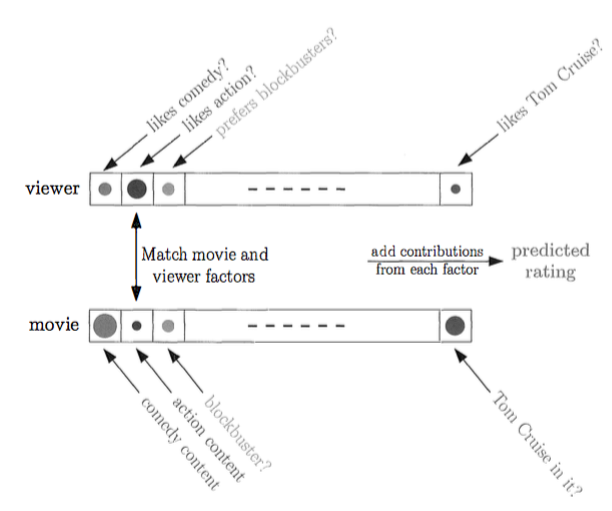
\includegraphics[width=0.8\textwidth]{include/netflix.png}
        \end{figure}
    \end{frame}

    \begin{frame}[t]{Dagens opgave}
        \begin{quote}
            Vi er blevet hyret af et hospital da de har hørt at vi dataloger
            kan hjælpe deres patienter.
        \end{quote}
        \pause
        \begin{block}{Problemstilling}
            Vi skal lave et system der, givet data om en patient, kan bestemme
            om deres svulst er godartet eller ondartet.
        \end{block}
        \pause
        \centering Hmm, det var da et ret generelt problem $\dots$
        \pause
        \begin{block}{Problemstilling}
            Vi skal lave et system der, givet data om en \alert{kunde},
            kan bestemme om det er en god forretning at låne dem penge.
        \end{block}
        \pause
        \centering Problemet hedder klassificering, gode løsninger kan have stor
        indflydelse inden for mange felter.
    \end{frame}

\section{Problemet}
\frame{\tableofcontents[currentsection]}
    \begin{frame}[c]{Håndtering af input og output}
        \begin{columns}
            \begin{column}{0.6\textwidth}
                \begin{block}{Input}
                    \begin{center}
                        \begin{tabular}{| c | r |}
                            \hline
                            Threshold                & 1           \\ \hline
                            Clump Thickness          & 7           \\ \hline
                            Uniformity of Cell Size  & 1           \\ \hline
                            Uniformity of Cell Shape & 4           \\ \hline
                            Epithelial Cell Size     & 2           \\ \hline
                            Bare Nuclei              & 3           \\ \hline
                            Bland Chromatin          & 8           \\ \hline
                            Normal Nucleoli          & 10          \\ \hline
                            Mitoses                  & 3           \\ \hline
                        \end{tabular}
                    \end{center}
                \end{block}
                \vspace{-1em}
                \begin{block}{Output}
                    \centering Ondartet eller godartet
                    {\color{KUNATgreen}1}
                \end{block}
            \end{column}
            \pause

            \begin{column}{0.1\textwidth}
                \vspace{4em}
                \begin{Huge}
                    $$
                        \rightarrow
                    $$
                \end{Huge}
            \end{column}
            \begin{column}{0.3\textwidth}
                \begin{block}{Data vektor}
                    $$
                        \left(
                        \begin{tabular}{c}
                            1      \\
                            7      \\
                            1      \\
                            4      \\
                            2      \\
                            3      \\
                            8      \\
                            10     \\
                            3
                        \end{tabular}
                        \right)
                    $$
                \end{block}
                \vspace{-1em}
                \begin{block}{Output}
                    1
                \end{block}
            \end{column}
        \end{columns}
    \end{frame}

    \begin{frame}[t]{Formalisering}
        \begin{block}{Termer}
            \begin{description}
                \item[Input] En vektor (patient data)  \pause
                \item[Output] $1$ eller $-1$ (ondartet eller godartet) \pause
                \item[Læringsmål]$\mathcal{F}: \mathcal{X} \rightarrow
                                   \mathcal{Y}$ \pause
                \item[Data] $(x_1,y_1), (x_2,y_2),\dots,(x_n,y_n)$
                (Hvad vi lærer fra) \pause
                \item[Hypotese] $g: \mathcal{X} \rightarrow
                                   \mathcal{Y}$ (Vores systems ``Hjerne'')
            \end{description}
        \end{block}
    \end{frame}

    \begin{frame}[c]{Visuel Formalisering}
        \begin{block}{~}
            \begin{figure}[h!]
                \caption{Visuelt læringsdiagram}
                \centering
                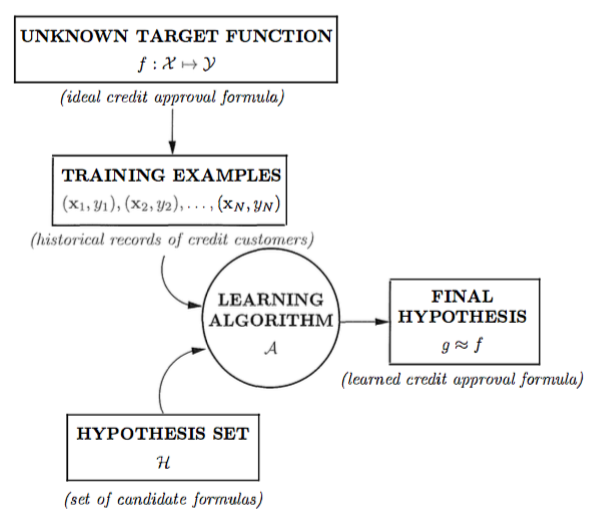
\includegraphics[width=0.7\textwidth]{include/dia.png}
            \end{figure}
        \end{block}
    \end{frame}


\section{Algoritmen}
\frame{\tableofcontents[currentsection]}

    \begin{frame}[t]{Valget af lærings-algoritmen}
        \begin{block}{Perceptron}
            Den laver et \emph{hyperplan} der adskiller data'en og finder en
            opdeling der giver en \alert{lav fejl}. \\
            \pause
            Tænk på den som en form for lineær regression på steroider
            $$
                y = ax + b
            $$
        \end{block}
        \pause
        \begin{block}{Eksempel på algoritmen}
            \begin{figure}[h!]
                \centering
                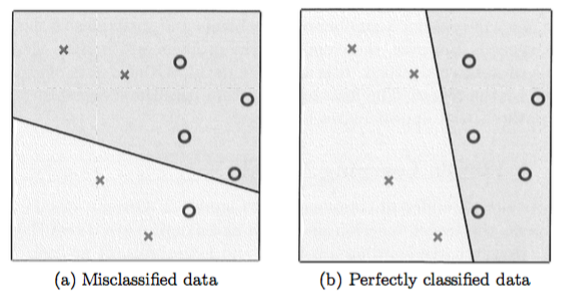
\includegraphics[width=0.6\textwidth]{include/per1.png}
            \end{figure}
        \end{block}
    \end{frame}


    \begin{frame}[t]{Algoritmen i ord}
        \begin{block}{Hvordan virker den?}
            Vi har en masse vektorer $v_1,v_2,\dots,v_n$ og en liste af svar
            $y_1,y_2,\dots,y_n$. \\
            \pause
            Vi lader $w$ være vores ``vægt-vektor''. \pause
            \vspace{-1em}
            \begin{flalign*}
                \text{Godartet svulst : } \sum_{i=1}^d w_i x_i &> b \\
                \text{Ondartet svulst : } \sum_{i=1}^d w_i x_i &< b
            \end{flalign*}
            \pause
            \vspace{-1em}
            Vores hypotese bliver så
            $$
                h(x) = fortegn\left(\sum_{i=0}^d w_i x_i \right)
            $$
            \pause
            \centering Men hvordan bestemmer vi $w$?
        \end{block}
    \end{frame}

    \begin{frame}[t]{Hvordan den lærer}
        \begin{block}{Hvordan $w$ bestemmes}
            \pause
            $$w = \text{ vælg tilfældige tal}$$
            \pause
            Vi forbedrer $w$ hver gang!\\ \pause
            Hvis $x'$ er på den forkerte side af $w$ så lærer den ``erfaringen''
            ved formlen \pause
            $$
                w_{ny} = w + y' x'
            $$
            \pause
            Forsæt med at lære indtil du ikke kan lære mere.
        \end{block}
    \end{frame}


    \begin{frame}[plain]{Perceptron algoritme}
        \begin{block}{Pseduocode}
        \vspace{-1.5em}
        \begin{algorithm}[H]
            \caption{\newline Input: datasæt $X=[(x_1,y_1),\dots, (x_n,y_n)]$
                     \newline Output: Hypotesen $w$.
            }
            \begin{algorithmic}
                \State w = Tilfældige tal
                \State misCat = $(1,1)$
                \While{$misCat \neq (0,0)$}
                \State misCat = $(0,0)$
                \For{$(x_i,y_i)$ in $X$}
                    \If{$sign(w^Tx_i) \neq y_i$ }
                        \State misCat = $(x_i,y_i)$
                        \State $w = w + y_i x_i$
                    \EndIf
                \EndFor
                \EndWhile \\
                \Return w
            \end{algorithmic}
        \end{algorithm}
        \end{block}
    \end{frame}

\section{Eksempel og algoritme-analyse}
\frame{\tableofcontents[currentsection]}
    \begin{frame}[t]{Vi prøver at køre den!}
        \begin{quote}
            Eksempel i MatLab
        \end{quote}
        \pause
        \begin{block}{Analyse}
            Nogen der kan gætte køretiden? \pause
            $$
                O(2^{(n+1) log(n+1)} (n + 1)^2)
            $$
                \pause
                Redder vi så nogle liv?
                \pause
                Lad os kode det og se hvor god den er!
            \end{block}
    \end{frame}

    \begin{frame}[t]{Afslutning}
    \begin{block}{Hvor god er den? }
        I opgaverne kigger i kun på alert{25 eksempler!} og tester på 75
        patienter \\
        \pause
        I kan forvente at den har ret på cirka $60-70\%$ af patienterne!.
        \pause
        Kører man den istedet med 500 eksempler og tester på 180. \pause
        Rammer den rigtigt 181 gange og forkert 2 gange. Det betyder at den
        har en succes rate på \alert{$98,9\%$!}
    \end{block}
    \pause
    \centering Spørgsmål?\\
    \end{frame}

    \begin{frame}[c]{Evaluering}
    \begin{block}{Facebook grupper}
        \centering
        https://www.facebook.com/DIKUDatalogi/ \\
        https://www.facebook.com/groups/Datalogi.I.Gymnasiet
    \end{block}
    \pause
    \begin{block}{Evaluerings skema}
        \centering
        http://rotendahl.dk/eval
    \end{block}
    \pause Tak for denne gang! (Vi ses på DIKU)
    \end{frame}


\end{document}
